\documentclass[border=3pt]{standalone}
% Preâmbulo compartilhado pelos diagramas TikZ da aula 5 de IHC (Processos de Design)
\usepackage[T1]{fontenc}
\usepackage[utf8]{inputenc}
\usepackage{lmodern}
\usepackage{amsmath}
\usepackage{xcolor}
\usepackage{tikz}
\usetikzlibrary{arrows.meta,angles,quotes,decorations.pathmorphing,calc,
                positioning,shapes.geometric,shapes.misc,backgrounds,fit,
                math}

% Paleta (mesma dos SVGs originais)
% Paleta da disciplina de IHC: acento roxo (#755099), da capa do livro.
% (o nome "dblue" é mantido para não alterar todos os diagramas)
\definecolor{dblue}{HTML}{755099}
\definecolor{dorange}{HTML}{B3541E}
\definecolor{dgreen}{HTML}{4A7C59}
\definecolor{dred}{HTML}{9C4B4B}
\definecolor{dcream}{HTML}{F4F1EA}
\definecolor{dshade}{HTML}{DDD7C9}

% Função gaussiana (não normalizada por padrão de escala visual)
\pgfmathdeclarefunction{gauss}{3}{%
  \pgfmathparse{1/(#3*sqrt(2*pi))*exp(-((#1-#2)^2)/(2*#3^2))}%
}

% Estilos comuns (prefixo d... para não colidir com chaves internas do pgf)
\tikzset{
  >={Stealth[length=2mm]},
  dguide/.style={gray!55, dashed, line width=0.4pt},
  daxis/.style={gray!60, line width=0.7pt, ->},
  dbody/.style={fill=black!3, draw=black!80, line width=1pt},
  dacc/.style={draw=dblue, line width=1pt},
  dlbl/.style={black!55, font=\small},
  dsub/.style={black!45, font=\footnotesize},
  dstate/.style={circle, draw=black!80, fill=dcream, line width=1pt,
                 minimum size=17mm, font=\large, inner sep=1pt},
  dobs/.style={circle, draw=black!80, fill=dshade, line width=1pt,
               minimum size=14mm, font=\large, inner sep=1pt},
  dbox/.style={rounded corners=2pt, draw=black!80, fill=dcream, line width=1pt,
               align=center, inner sep=6pt},
  dop/.style={circle, draw=black!80, fill=white, line width=1pt,
              minimum size=6mm, inner sep=0pt, font=\small},
  dtrans/.style={->, dblue, line width=1pt},
  dmeas/.style={->, dorange, line width=1pt},
  dcurve/.style={line width=1pt, dblue},
  dcurveb/.style={line width=1.4pt, dorange},
}

\begin{document}
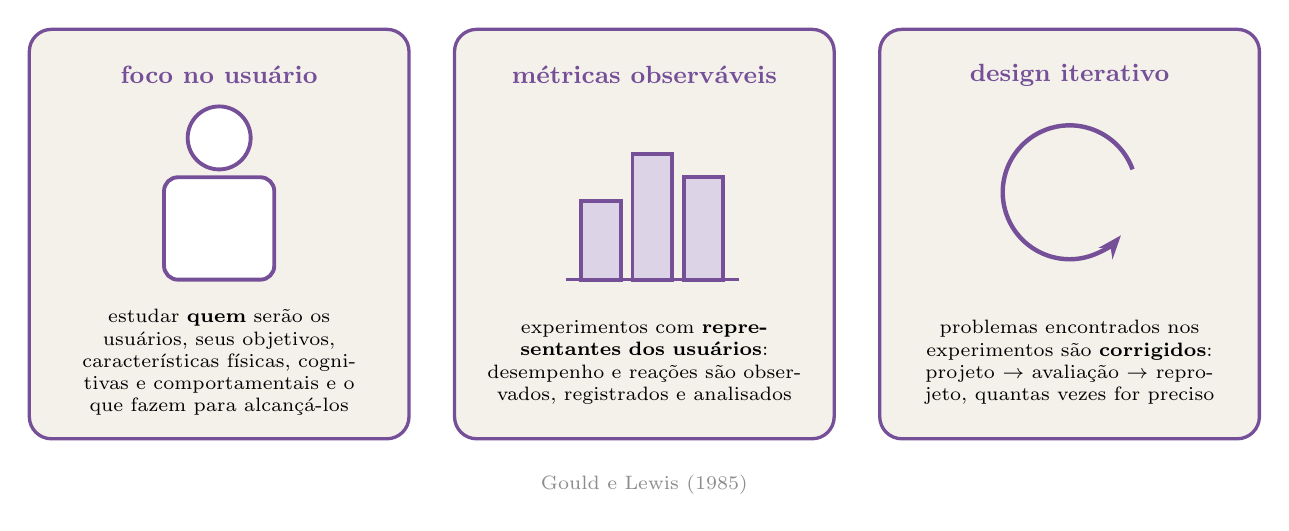
\begin{tikzpicture}[x=1cm,y=1cm,
   col/.style={dbox, rounded corners=8pt, text width=4.4cm, minimum height=5.2cm, anchor=north, align=center, font=\scriptsize}]

  \foreach \x in {0,5.4,10.8} { \node[col, draw=dblue, line width=1.2pt] at (\x,0) {}; }

  % 1 foco no usuário
  \begin{scope}[shift={(0,-2.3)}]
    \draw[dblue, line width=1.4pt, fill=white] (0,0.9) circle (0.4);
    \draw[dblue, line width=1.4pt, fill=white, rounded corners=5pt] (-0.7,-0.9) rectangle (0.7,0.4);
  \end{scope}
  \node[font=\small\bfseries, dblue] at (0,-0.6) {foco no usuário};
  \node[text width=4.0cm, align=center, font=\scriptsize] at (0,-4.25) {estudar \textbf{quem} serão os usuários, seus objetivos, características físicas, cognitivas e comportamentais e o que fazem para alcançá-los};

  % 2 métricas observáveis
  \begin{scope}[shift={(5.4,-2.4)}]
    \draw[dblue, line width=1.4pt, fill=dblue!25] (-0.8,-0.8) rectangle (-0.3,0.2);
    \draw[dblue, line width=1.4pt, fill=dblue!25] (-0.15,-0.8) rectangle (0.35,0.8);
    \draw[dblue, line width=1.4pt, fill=dblue!25] (0.5,-0.8) rectangle (1.0,0.5);
    \draw[dblue, line width=1.2pt] (-1.0,-0.8) -- (1.2,-0.8);
  \end{scope}
  \node[font=\small\bfseries, dblue] at (5.4,-0.6) {métricas observáveis};
  \node[text width=4.0cm, align=center, font=\scriptsize] at (5.4,-4.25) {experimentos com \textbf{representantes dos usuários}: desempenho e reações são observados, registrados e analisados};

  % 3 design iterativo
  \begin{scope}[shift={(10.8,-2.2)}]
    \draw[dblue, line width=1.6pt, -{Stealth[length=3mm]}] (0.8,0.4) arc (20:320:0.85);
  \end{scope}
  \node[font=\small\bfseries, dblue] at (10.8,-0.6) {design iterativo};
  \node[text width=4.0cm, align=center, font=\scriptsize] at (10.8,-4.25) {problemas encontrados nos experimentos são \textbf{corrigidos}: projeto $\to$ avaliação $\to$ reprojeto, quantas vezes for preciso};

  \node[dsub, font=\scriptsize] at (5.4,-5.8) {Gould e Lewis (1985)};

\end{tikzpicture}
\end{document}
